\chapter{Valutazione euristica} \label{chap:valutazione_euristica}

	Il metodo della valutazione euristica è un metodo sviluppato da Jakob Nielsen per la valutazione dell'usabilità di un'interfaccia. Questo metodo consiste nel seguire delle linee guida, dette ``euristiche'', per determinare i problemi di usabilità di un'interfaccia.\\
	Le euristiche, proposte da Nielsen stesso, sono 10. La prima formulazione del metodo risale a molti anni fa ed era pensata per interfacce software. Col passare degli anni, tuttavia, le euristiche sono state riviste e corrette e, con l'avvento del Web, è stata proposta anche una versione per valutare l'usabilità dei siti web.\\
	\\
	Le 10 euristiche di Nielsen sono:
	\begin{enumerate}
		\item Visibilità dello stato del sistema
		\item Corrispondenza tra sistema e mondo reale
		\item Controllo e libertà
		\item Consistenza e standard
		\item Prevenzione dell'errore
		\item Riconoscimento anziché ricordo
		\item Flessibilità d'uso
		\item Design ed estetica minimalista
		\item Aiuto all'utente
		\item Documentazione
	\end{enumerate}
	
	Vediamo nel dettaglio cosa rappresenta ogni euristica e come viene valutata l'interfaccia di Gmail e Yahoo Mail rispetto ad ognuna di esse.
	
	\section{Visibilit\`{a} dello stato del sistema} \label{sec:visibilità_stato_sistema}
	
		La prima euristica di Nielsen per lo studio dell'usabilità di siti Web afferma che:
		\begin{center}
			\begin{minipage}{0.7\textwidth}
				\textit{``Il sistema deve costantemente informare l'utente su ciò che sta succedendo, fornendo appropriato feedback in tempi ragionevoli.''}
			\end{minipage}
		\end{center}
		
		Andiamo a vedere come si comportano, in questo senso, Gmail e Yahoo Mail.\\
		\\
		Innanzitutto\marginpar{Caricamento}, all'apertura della casella di posta, si nota subito come la pagina di Gmail venga aperta subito, mostrando la barra di caricamento in Figura \ref{fig:caricamento_gmail}, mentre con Yahoo Mail il browser resterà in attesa fino al caricamento dell'intera pagina.
		\begin{figure}[h!]
			\begin{center}
				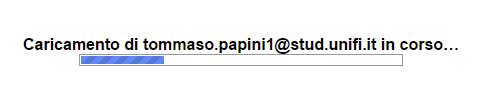
\includegraphics[scale=1]{caricamento_gmail.png}
			\end{center}
			\caption[Caricamento in Gmail]{Caricamento della casella di posta Gmail.}
			\label{fig:caricamento_gmail}
		\end{figure}
		
		Questo secondo approccio è sconsigliato in quanto, durante il tempo necessario al caricamento della pagina, l'utente potrebbe domandarsi se la sua casella di posta si stia effettivamente caricando: \textit{``forse il sito non è raggiungibile? forse il server di Yahoo Mail è momentaneamente down? forse ho inserito male l'indirizzo?''} L'utente non ha ben chiaro cosa stia succedendo e questo può portare a fraintendimenti e frustrazione.\\
		\\
		
		Una\marginpar{Titolo} volta caricata la casella di posta, ci soffermiamo invece sul titolo della pagina. Nel caso di Yahoo Mail il titolo è unico e statico, come possiamo vedere ad esempio in Figura \ref{fig:titolo_yahoo}.
		\begin{figure}[h!]
			\begin{center}
				
\includegraphics[scale=1]{titolo_yahoo.png}
			\end{center}
			\caption[Titolo di Yahoo Mail]{Titolo di tutte le pagine di Yahoo Mail.}
			\label{fig:titolo_yahoo}
		\end{figure}
		
		Gmail al contrario aggiunge, al titolo di base, la cartella correntemente visitata o l'oggetto della mail aperta, come possiamo vedere in Figura \ref{fig:titoli_gmail}.
		\begin{figure}[h!]
			\begin{center}
				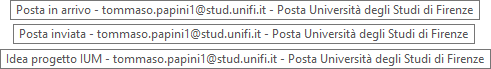
\includegraphics[scale=1]{titoli_gmail.png}
			\end{center}
			\caption[Titoli di Gmail]{Alcuni titoli delle pagine di Gmail.}
			\label{fig:titoli_gmail}
		\end{figure}
		\\
		
		In\marginpar{Struttura} entrambi i casi, la struttura della casella di posta è piuttosto chiara e ben organizzata: su una colonna a sinistra troviamo le varie cartelle della posta (In arrivo, Inviata, Bozze, ecc\dots), mentre in alto troviamo le azioni sulle mail (a sinistra) e le impostazioni dell'account (a destra), il tutto sovrastato da un campo di ricerca, per poter cercare sia all'interno della casella di posta che sul Web. Nel centro si trova invece una grande colonna contenente i messaggi della cartella selezionata, ordinati e/o filtrati secondo i criteri scelti dall'utente.\\
		\\
		Un\marginpar{Invio} altro caso di visibilità dello stato del sistema si ha quando si invia un nuovo messaggio di posta elettronica (sia che sia scritto da zero o come risposta/inoltro). Nel caso di Gmail si ha, come si può vedere in Figura \ref{fig:msg_invio_gmail}, che il sito mostra all'utente, in modo non intrusivo, due messaggi, dove viene indicato che si sta inviando la mail e dove si conferma l'avvenuto invio.
		\begin{figure}[h!]
			\begin{center}
				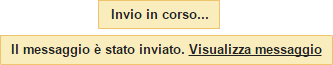
\includegraphics[scale=1]{msg_invio_gmail.png}
			\end{center}
			\caption[Messaggi d'invio in Gmail]{I messaggi visualizzati da Gmail all'invio di una nuova email.}
			\label{fig:msg_invio_gmail}
		\end{figure}
		
		In questo modo l'utente sarà sempre al corrente di quello che sta facendo Gmail. Per Yahoo Mail il discorso è molto simile. L'unica differenza si ha per il messaggio d'attesa mentre si sta inviando la mail: in questo caso non viene visualizzato un box in stile popup, ma appare la scritta ``Invio'' in basso alla finestra di composizione della mail, affiancata ad un'animazione che ricorda una ``rotella'' che gira, ad indicare che Yahoo Mail sta lavorando per eseguire l'invio (Figura \ref{fig:msg_invio_yahoo}).
		\begin{figure}[h!]
			\begin{center}
				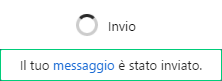
\includegraphics[scale=1]{msg_invio_yahoo.png}
			\end{center}
			\caption[Messaggi d'invio in Yahoo Mail]{I messaggi visualizzati da Yahoo Mail all'invio di una nuova email.}
			\label{fig:msg_invio_yahoo}
		\end{figure}
		
		I due approcci sono molto simili (ed uguali quando il messaggio è stato inviato) e forniscono allo stesso modo un'idea chiara di quello che sta succedendo una volta terminato di scrivere una mail.\\
		\\
		Un\marginpar{Salvataggio\\bozza} altro messaggio utile mostrato all'utente è quello del salvataggio della bozza che si sta scrivendo. Gmail visualizza due semplici messaggi (Figura \ref{fig:msg_bozza_gmail}) in basso alla finestra di composizione, in modo simile a quanto visto per i messaggi d'invio.
		\begin{figure}[h!]
			\begin{center}
				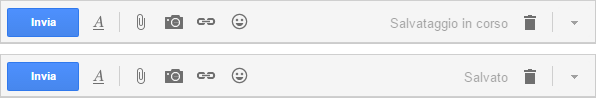
\includegraphics[scale=0.8]{msg_bozza_gmail.png}
			\end{center}
			\caption[Messaggi di salvataggio bozza in Gmail]{I messaggi visualizzati da Gmail al salvataggio di una bozza.}
			\label{fig:msg_bozza_gmail}
		\end{figure}
		
		Anche Yahoo Mail mostra dei messaggi in modo molto simile a quanto fatto da Gmail (Figura \ref{fig:msg_bozza_yahoo}), anche se si è riscontrato che mentre Gmail visualizza il messaggio non appena si effettuano delle modifiche, Yahoo Mail aspetta che trascorra un certo lasso di tempo senza modifiche prima di visualizzare i messaggi.
		\begin{figure}[h!]
			\begin{center}
				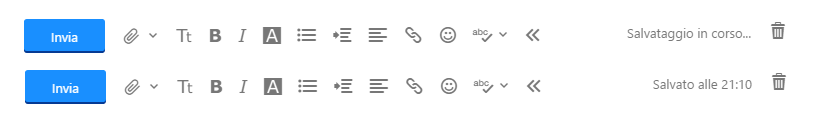
\includegraphics[scale=0.6]{msg_bozza_yahoo.png}
			\end{center}
			\caption[Messaggi di salvataggio bozza in Yahoo Mail]{I messaggi visualizzati da Yahoo Mail al salvataggio di una bozza.}
			\label{fig:msg_bozza_yahoo}
		\end{figure}
		
		Cosa accade in quel lasso di tempo? Se si chiude improvvisamente la composizione mail in quel periodo la mail viene persa o salvata? L'utente potrebbe rimanere incerto sulla fine della sua bozza, quindi in questo caso un'interfaccia più reattiva come quella di Gmail può fare la differenza.\\
		\\
		Sempre\marginpar{Aggiunta\\allegato} sull'argomento dei messaggi informativi, si possono considerare i messaggi durante l'aggiunta di un allegato ad una mail. Gmail mostra una barra progressiva durante l'upload, come si vede in Figura \ref{fig:msg_allegato_gmail}, e quindi il nome dell'allegato evidenziato di blu (ad indicare che è un link per scaricare l'allegato stesso) una volta aggiunto.
		\begin{figure}[h!]
			\begin{center}
				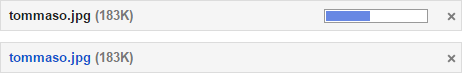
\includegraphics[scale=1]{msg_allegato_gmail.png}
			\end{center}
			\caption[Messaggi all'aggiunta di un allegato in Gmail]{I messaggi visualizzati da Gmail all'aggiunta di un nuovo allegato.}
			\label{fig:msg_allegato_gmail}
		\end{figure}
		
		Yahoo Mail invece mostra un messaggio sopra all'anteprima del file (se disponibile) con a fianco una rotellina che gira ed una barra progressiva verde in basso (Figura \ref{fig:msg_allegato_yahoo}), mentre una volta aggiunto l'allegato mostra soltanto l'anteprima.
		\begin{figure}[h!]
			\begin{center}
				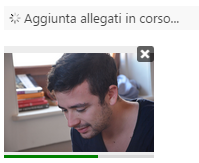
\includegraphics[scale=1]{msg_allegato_yahoo.png}
			\end{center}
			\caption[Messaggio all'aggiunta di un allegato in Yahoo Mail]{Il messaggio visualizzato da Yahoo Mail all'aggiunta di un nuovo allegato.}
			\label{fig:msg_allegato_yahoo}
		\end{figure}
		
		Entrambi i messaggi sono piuttosto chiari, anche se la barra progressiva utilizzata da Gmail viene mostrata sempre, mentre su Yahoo Mail soltanto per file più grandi. L'approccio di Gmail è in generale preferibile in quanto si da sempre l'idea del caricamento progressivo del file sul messaggio, anche se tale caricamento è pressoché immediato (e anche per un discorso di consistenza).\\
		\\
		Un\marginpar{Etichette} altro aspetto importante sono le etichette. Parleremo più ampiamente delle etichette e dell'organizzazione delle mail nelle Sezioni \ref{sec:controllo_libertà} e \ref{sec:flessibilità_uso}, ma è giusto fare un accenno anche per questa prima euristica. Le etichette delle mail rappresentano un modo di organizzare i messaggi in una o più categorie a seconda di vari criteri scelti dall'utente. In Yahoo Mail non c'è un vero e proprio supporto alle etichette, ma soltanto alle cartelle (ogni mail sta in una sola cartella ma può avere più etichette). A parte questa mancanza di Yahoo Mail, che analizzeremo in dettaglio nella Sezione \ref{sec:flessibilità_uso}, Yahoo Mail non mostra in alcun modo all'interno della mail a quale cartella essa appartenga. L'unico modo che ha l'utente di sapere se una mail appartiene ad una cartella anziché ad un'altra è di guardare il menù a sinistra e cercare la voce evidenziata.\\
		In Gmail invece, come vediamo in Figura \ref{fig:etichette_gmail}, accanto al titolo della mail aperta vengono visualizzate tutte le etichette assegnate a tale mail.
		\begin{figure}[h!]
			\begin{center}
				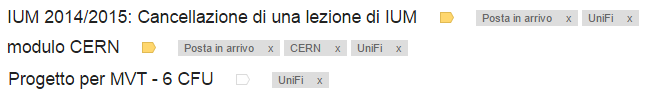
\includegraphics[scale=0.8]{etichette_gmail.png}
			\end{center}
			\caption[Etichette in Gmail]{Alcuni esempi di etichette in Gmail.}
			\label{fig:etichette_gmail}
		\end{figure}
		
		In questo modo l'utente saprà sempre a quale/i categoria/e appartiene la mail che sta leggendo. Inoltre sarà possibile cliccare su un'etichetta per saltare all'elenco di tutte le mail con la stessa etichetta (ne parleremo in Sezione \ref{sec:controllo_libertà}). Purtroppo l'unica pecca di Gmail in questo senso è di non riconoscere ``Posta inviata'' come etichetta, mostrando soltanto il resto delle etichette.\\
		\\
		Per il resto, come si è già detto, la struttura delle due caselle di posta è molto chiara e intuitiva: i pulsanti, i link e i campi da riempire sono facilmente riconoscibili tra loro e difficilmente possono indurre l'utente a perdersi all'interno della pagina.\\
		\\
		Per quanto esposto in questa Sezione, assegnamo adesso un voto in decimi ad entrambe le caselle di posta riguardo la prima euristica.
		
		\begin{flushleft}
			\begin{tabular}{lr}
				\textsc{Gmail} & $9/10$\\
				\textsc{Yahoo Mail} & $7/10$
			\end{tabular}
		\end{flushleft}
	
	\section{Corrispondenza tra sistema e mondo reale} \label{sec:corrispondenza_sistema_mondo_reale}
	
		La seconda euristica di Nielsen afferma che:
		\begin{center}
			\begin{minipage}{0.7\textwidth}
				\textit{``Il sistema deve parlare il linguaggio dell'utente con parole, frasi e concetti a lui familiari.''}
			\end{minipage}
		\end{center}
		
		La\marginpar{Icone} prima cosa che viene in mente in questo senso sono le icone. In entrambi i casi le icone utilizzate sono piuttosto intuitive e seguono le common practices (standard de facto) ormai stabilitesi sul Web. Alcuni esempi sono le classiche icone del cestino per eliminare un oggetto, la graffetta per aggiungere un allegato o la catena per inserire un collegamento ipertestuale. A titolo d'esempio si vedano le Figure \ref{fig:icone_gmail} e \ref{fig:icone_yahoo}.
		\begin{figure}[h!]
			\begin{center}
				
\includegraphics[scale=1]{icone_gmail.png}
			\end{center}
			\caption[Icone di Gmail]{Alcune icone utilizzate in Gmail.}
			\label{fig:icone_gmail}
		\end{figure}
		\begin{figure}[h!]
			\begin{center}
				
\includegraphics[scale=1]{icone_yahoo.png}
			\end{center}
			\caption[Icone di Yahoo Mail]{Alcune icone utilizzate in Yahoo Mail.}
			\label{fig:icone_yahoo}
		\end{figure}
		\\
		
		L'altro\marginpar{Linguaggio} aspetto importante per garantire corrispondenza tra il sistema ed il mondo reale è utilizzare un linguaggio adatto all'utente, o perlomeno al target di utenti previsto. Questo implica dare nomi appropriati ai vari link e bottoni in modo che l'utente sappia sempre di cosa si sta parlando e che funzione svolgono i vari elementi della pagina. In questo senso entrambi i provider utilizzano nomi piuttosto comuni sul Web e che richiamano al linguaggio naturale dell'utente: ad esempio etichette come ``Posta in arrivo'', ``Bozze'' o ``Posta inviata'' sono molto esplicative e lasciano ben poco spazio a fraintendimenti. Se proprio si vuol fare una distinzione tra i due sistemi, possiamo notare che mentre Gmail utilizza l'etichetta ``Spam'' per la posta indesiderata e ``Speciali''/``Importanti'' per i messaggi più importanti, Yahoo Mail utilizza, rispettivamente, ``Antispam'' e ``Con stella''. Il caso spam/antispam può creare confusione tra gli utenti (specialmente se non pratici della lingua inglese) in quanto le due etichette sembrano indicare cose opposte tra loro. Se proprio si deve decidere una delle due soluzioni, probabilmente ``Spam'' è preferibile, in quanto l'etichetta di una cartella dovrebbe indicare cosa vi è dentro (ovvero spam) e non perché o cosa ce l'ha messo (il sistema di antispam). Per sistemi che, come questi, supportano la lingua italiana sarebbe preferibile optare per un ``Posta indesiderata'' per fugare ogni dubbio. Anche l'etichetta ``Con stella'' può causare qualche perplessità: è vero che per ``convenzione'' si utilizza un simbolino fatto a stella per contrassegnare i messaggi importanti, ma un utente inesperto potrebbe chiedersi cosa possa rappresentare un messaggio ``con stella'', finendo per trascurare questa funzionalità.\\
		\\
		Tirando le somme per quest'euristica, assegnamo adesso un voto, come fatto nella Sezione precedente, ai due servizi di posta elettronica.
		
		\begin{flushleft}
			\begin{tabular}{lr}
				\textsc{Gmail} & $10/10$\\
				\textsc{Yahoo Mail} & $9/10$
			\end{tabular}
		\end{flushleft}
	
	\section{Controllo e libert\`{a}} \label{sec:controllo_libertà}
	
		Vediamo adesso la terza euristica di Nielsen per i siti Web. Essa afferma che:
		\begin{center}
			\begin{minipage}{0.7\textwidth}
				\textit{``L'utente deve avere il controllo del contenuto informativo e muoversi liberamente tra i vari argomenti.''}
			\end{minipage}
		\end{center}
		
		Quindi è chiaro che quest'euristica si occupa della buona navigabilità all'interno del sito Web. Concetti chiave in questo senso sono il supporto o meno di tasti rapidi, la possibilità di navigare con tastiera e la presenza di un tasto ``Indietro''. Esaminiamo questi aspetti uno per uno.\\
		\\
		I\marginpar{Tasti rapidi} tasti rapidi, o tasti di scelta rapida, rappresentano quelle combinazioni da tastiera che permettono di eseguire in modo più rapido un'azione frequente. Gmail, ad esempio, permette all'utente di selezionare, con apposite combinazioni, le azioni più frequenti durante la composizione di una nuova mail: passando il mouse sul bottone corrispondente, Gmail mostrerà l'azione del bottone e la combinazione da tastiera corrispondente, come in Figura \ref{fig:tasti_rapidi_gmail}.
		\begin{figure}[h!]
			\begin{center}
				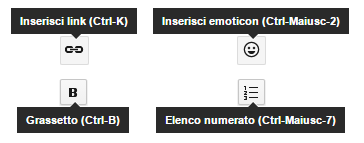
\includegraphics[scale=1]{tasti_rapidi_gmail.png}
			\end{center}
			\caption[Tasti rapidi di Gmail]{Alcuni tasti di scelta rapida in Gmail.}
			\label{fig:tasti_rapidi_gmail}
		\end{figure}
		
		Tuttavia, mentre Gmail mappa tutti i pulsanti presenti e rende le combinazioni assegnate visibili all'utente, Yahoo Mail prevede l'utilizzo soltanto di alcuni tasti di scelta rapida, come per la scrittura in grassetto o in corsivo, tralasciando gli altri pulsanti, e anche le poche combinazioni presenti non vengono rese chiare all'utente.\\
		\\
		La\marginpar{Tastiera} navigazione da tastiera è implementata in entrambi i provider di posta, anche se in modo diverso. Ad esempio è possibile scorrere la lista dei messaggi, in entrambi i siti, utilizzando le frecce della tastiera. Tuttavia, quando si apre una mail e si vuole tornare indietro a dove eravamo prima, in Gmail si utilizza il tasto Back (consistente con quanto fatto dal browser normalmente) mentre in Yahoo Mail si utilizza Esc. L'utilizzo del tasto Esc può forse confondere in quanto normalmente viene utilizzato per chiudere qualcosa e non per tornare indietro. Infatti in Gmail si utilizza Esc quando si vuole chiudere una mail in composizione, in quanto essa appare come finestra sovrapposta alla vista corrente e non in sostituzione.\\
		\\
		Il\marginpar{Indietro} tasto Indietro serve quando si apre una mail e si vuole tornare alla cartella di partenza. Gmail implementa un tasto Indietro in ogni mail, posizionato in alto a sinistra, accanto alle altre azioni sulla mail (Figura \ref{fig:indietro_gmail}).
		\begin{figure}[h!]
			\begin{center}
				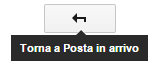
\includegraphics[scale=1]{indietro_gmail.png}
			\end{center}
			\caption[Tasto Indietro in Gmail]{Il tasto Indietro presente in Gmail.}
			\label{fig:indietro_gmail}
		\end{figure}
		
		C'è da osservare come il tasto Indietro in Gmail sia leggermente più difficile da implementare rispetto a quello di Yahoo Mail in quanto quest'ultimo dovrebbe soltanto ricondurre alla cartella di appartenenza (unica) senza doversi ricordare da quale cartella si era venuti (necessario in Gmail per via delle etichette). Siamo infatti rimasti piuttosto perplessi nel vedere che Yahoo Mail non implementa affatto un bottone Indietro. Su Yahoo Mail c'è, in ogni mail, un bottone molto simile e nella stessa posizione di quello di Gmail, che tuttavia non serve a tornare indietro, ma bensì a rispondere al mittente (Figura \ref{fig:indietro_yahoo}), cosa inutile e ridondante visto che Yahoo Mail, come Gmail, ha già una casella di testo sotto al corpo della mail per comporre una risposta.
		\begin{figure}[h!]
			\begin{center}
				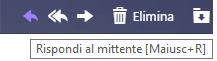
\includegraphics[scale=1]{indietro_yahoo.png}
			\end{center}
			\caption[Finto tasto Indietro in Yahoo Mail]{Il ``finto'' tasto Indietro presente in Yahoo Mail.}
			\label{fig:indietro_yahoo}
		\end{figure}
		
		D'altro canto, si potrebbe pensare che un tasto Indietro dedicato sia inutile, dal momento che ormai qualsiasi browser in circolazione implementa un suo tasto Indietro per navigare attraverso la cronologia Web. Peccato che Yahoo Mail non supporti pienamente nemmeno l'Indietro del browser: spesso è necessario cliccare Indietro due o più volte per tornare effettivamente indietro, mentre altre volte non funziona affatto (come quando si sta componendo una nuova mail). Esula dagli obiettivi di questo capitolo valutare un sito in base a quanto bene esso si interfacci con i browser, ma a nostro parere il fatto che il tasto Indietro del browser non sia pienamente supportato è una ragione in più per fornire un tasto Indietro dedicato. Gmail, al contrario, supporta pienamente anche il tasto Indietro del browser.\\
		\\
		Come\marginpar{Etichette} già accennato nella Sezione \ref{sec:visibilità_stato_sistema}, Gmail utilizza un sistema molto utile di etichette per contrassegnare i messaggi in vari modi, mentre Yahoo Mail soltanto un sistema di cartelle. In Figura \ref{fig:etichette_gmail} (a pagina \pageref{fig:etichette_gmail}) vediamo come ogni volta che apriamo un messaggio in Gmail esso visualizzi accanto all'oggetto tutte le etichette associate a tale mail. Queste etichette non servono soltanto ad informare l'utente sul tipo (o tipi) di mail che si sta leggendo, ma servono anche come strumento di navigazione veloce: cliccando su una qualsiasi etichetta, infatti, l'utente verrà portato alla lista di tutte le mail appartenenti a quella categoria, ovvero aventi in comune la stessa etichetta selezionata. Questa funzionalità è assente in Yahoo Mail in quanto qualora un utente voglia selezionare la stessa cartella (in assenza di etichette) dovrà necessariamente andare a cercare la voce corrispondente sul menù a sinistra, in mezzo a tutte le altre cartelle.\\
		\\
		Per il resto, entrambi i siti implementano le cose più comuni in fatto di navigazione: entrambi presentano un link alla home page in alto a sinistra della pagina (corrispondente col logo), entrambi permettono di scaricare un allegato appena aggiunto con un semplice click ed entrambi permettono di visualizzare il testo di una mail mentre si stanno ancora caricando gli allegati.\\
		\\
		In conclusione, per quanto riguarda la navigazione, non c'è niente da dire a Gmail, mentre Yahoo Mail potrebbe adottare alcuni accorgimenti che lo renderebbero sicuramente più usabile.
		
		\begin{flushleft}
			\begin{tabular}{lr}
				\textsc{Gmail} & $10/10$\\
				\textsc{Yahoo Mail} & $6/10$
			\end{tabular}
		\end{flushleft}
	
	\section{Consistenza e standard} \label{sec:consistenza_standard}
	
		Parliamo adesso di consistenza e standard di un sito Web.
		\begin{center}
			\begin{minipage}{0.7\textwidth}
				\textit{``L'utente deve aspettarsi che le convenzioni del sistema siano valide per tutte le pagine del sito.''}
			\end{minipage}
		\end{center}
		
		Riguardo a quest'euristica, fortunatamente, non c'è molto da dire. Entrambi i provider di posta sono consistenti con se stessi e con le varie convenzioni del Web. Entrambi i siti utilizzano una combinazione di stili, colori e font che viene mantenuta all'interno di tutto il sito, in modo da rendere la casella di posta consistente a livello stilistico. Anche le convenzioni del Web vengono rispettate: la struttura del sito è quella della tipica casella di posta, con i menù a sinistra e l'elenco delle mail nel centro, e le icone seguono le convenzioni in vigore sul Web (si vedano le Figure \ref{fig:icone_gmail} e \ref{fig:icone_yahoo}).
		
		\begin{flushleft}
			\begin{tabular}{lr}
				\textsc{Gmail} & $10/10$\\
				\textsc{Yahoo Mail} & $10/10$
			\end{tabular}
		\end{flushleft}
	
	\section{Prevenzione dell'errore} \label{sec:prevenzione_errore}
	
		Vediamo adesso la quinta euristica. Essa afferma che bisogna:
		\begin{center}
			\begin{minipage}{0.7\textwidth}
				\textit{``Evitare di porre l'utente in situazioni ambigue, critiche, che possono portare all'errore.''}
			\end{minipage}
		\end{center}
		
		Diciamo subito che in entrambi i siti di posta elettronica analizzati è difficile produrre errori. Questo perché, come già detto nella Sezione \ref{sec:visibilità_stato_sistema}, la struttura priva di frame di questi siti è chiara e solida e permette all'utente di fare, in ogni momento, tutte e sole le operazioni consentite, garantendo liberà di navigazione ma allo stesso tempo limitando gli errori. Ad esempio non si troveranno mai link (intra-sito) non definiti o pagine senza sfondo: grazie al menù di navigazione si ha accesso in qualsiasi istante a tutte le cartelle della nostra casella. Inoltre, come già visto in Sezione \ref{sec:corrispondenza_sistema_mondo_reale}, le etichette dei vari comandi e link sono chiare e esplicative e i vari elementi d'interazione sono facilmente riconoscibili, lasciando poco spazio a fraintendimenti.\\
		\\
		Entrambi\marginpar{Form} i siti forniscono anche suggerimenti visivi per la correzione di campi di form prima del loro invio. Se ad esempio inseriamo un indirizzo di posta con un formato sbagliato (ad esempio senza chiocciola) mentre componiamo una nuova mail, esso verrà sottolineato (in Gmail, Figura \ref{fig:errore_indirizzo_gmail}) o evidenziato (in Yahoo Mail, Figura \ref{fig:errore_indirizzo_yahoo}) in rosso.
		\begin{figure}[h!]
			\begin{center}
				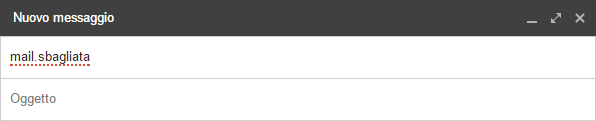
\includegraphics[scale=0.8]{errore_indirizzo_gmail.png}
			\end{center}
			\caption[Errore indirizzo in Gmail]{Feedback visivo per un formato scorretto dell'indirizzo in Gmail.}
			\label{fig:errore_indirizzo_gmail}
		\end{figure}
		\begin{figure}[h!]
			\begin{center}
				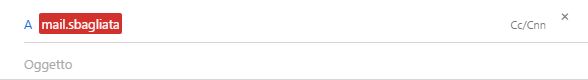
\includegraphics[scale=0.8]{errore_indirizzo_yahoo.png}
			\end{center}
			\caption[Errore indirizzo in Yahoo Mail]{Feedback visivo per un formato scorretto dell'indirizzo in Yahoo Mail.}
			\label{fig:errore_indirizzo_yahoo}
		\end{figure}
		\\
		
		Possiamo\marginpar{URL} tuttavia fare una piccola osservazione riguardo agli URL del sito. Utilizzare URL semplici, corti ed autoesplicativi permette all'utente di orientarsi più facilmente all'interno del sito ed evitare di confondersi tra link simili. In Gmail, come si vede nella Tabella \ref{tab:url_gmail}, l'utente si ritrova davanti dei link molto brevi e compatti e con significato ovvio: ``inbox'' è il nome in inglese per la posta in arrivo, ``sent'' significa ``(posta) inviata'' in inglese, e così via.
		\begin{table}[h!]
			\centering
			\begin{tabular}{|l|l|}
				\hline
				\multicolumn{1}{|c|}{\textbf{Pagina}}& \multicolumn{1}{c|}{\textbf{URL Gmail}}\\ \hline\hline
				Posta in arrivo & \url{.../mail/u/1/#inbox}\\ \hline
				Posta inviata & \url{.../mail/u/1/#sent}\\ \hline
				Scrivi & \url{.../mail/u/1/#inbox?compose=new}\\ \hline
			\end{tabular}
			\caption[URL in Gmail]{Esempi di URL in Gmail.}
			\label{tab:url_gmail}
		\end{table}
		
		Anche l'URL di base di Gmail (nella tabella omesso con dei puntini) è molto semplice: \url{https://mail.google.com}.\\
		\\
		In Yahoo Mail invece, come vediamo nella Tabella \ref{tab:url_yahoo}, gli URL sono più lunghi rispetto a Gmail e il loro significato non è deducibile a priori: sono infatti formati da una stringa alfanumerica, che identifica la sessione corrente, e un numero a 10 cifre indicante la cartella o mail visitata.
		\begin{table}[h!]
			\centering
			\begin{tabular}{|l|l|}
				\hline
				\multicolumn{1}{|c|}{\textbf{Pagina}}& \multicolumn{1}{c|}{\textbf{URL Yahoo Mail}}\\ \hline\hline
				Posta in arrivo & \url{.../neo/launch?.rand=3k9uet4htd1q2#4928239615}\\ \hline
				Posta inviata & \url{.../neo/launch?.rand=3k9uet4htd1q2#3092874305}\\ \hline
				Scrivi & \url{.../neo/launch?.rand=3k9uet4htd1q2#6440717164}\\ \hline
			\end{tabular}
			\caption[URL in Yahoo Mail]{Esempi di URL in Yahoo Mail.}
			\label{tab:url_yahoo}
		\end{table}
		
		Non solo non è possibile capire, dal solo URL, quale pagina si stia visitando, ma questi URL cambiano ogni volta che si ricarica la pagina (come suggerito dal nome ``rand'' del campo della query) rendendo impossibile riutilizzare gli stessi URL in futuro per un accesso rapido. Anche l'URL di base di Yahoo Mail risulta meno chiaro rispetto a quello di Gmail: \url{https://it-mg42.mail.yahoo.com}.\\
		\\
		Tirando le somme, assegnamo un voto ai due provider anche per quest'euristica.
		
		\begin{flushleft}
			\begin{tabular}{lr}
				\textsc{Gmail} & $10/10$\\
				\textsc{Yahoo Mail} & $9/10$
			\end{tabular}
		\end{flushleft}
	
	\section{Riconoscimento anzich\'{e} ricordo} \label{sec:riconoscimento_anziché_ricordo}
	
		La sesta euristica dice che:
		\begin{center}
			\begin{minipage}{0.7\textwidth}
				\textit{``La navigazione deve essere ben visibile e facilmente accessibile.''}
			\end{minipage}
		\end{center}
		
		Supponiamo\marginpar{Elenco\\mail} di considerare le varie mail come possibili ``link''. La visualizzazione iniziale in Gmail non può essere definita pesante perché ogni mail ha un'ampiezza di circa 1 cm che consente di non far appesantire la schermata iniziale, come possiamo vedere in Figura \ref{fig:lista_mail_gmail}.
		\begin{figure}[h!]
			\begin{center}
				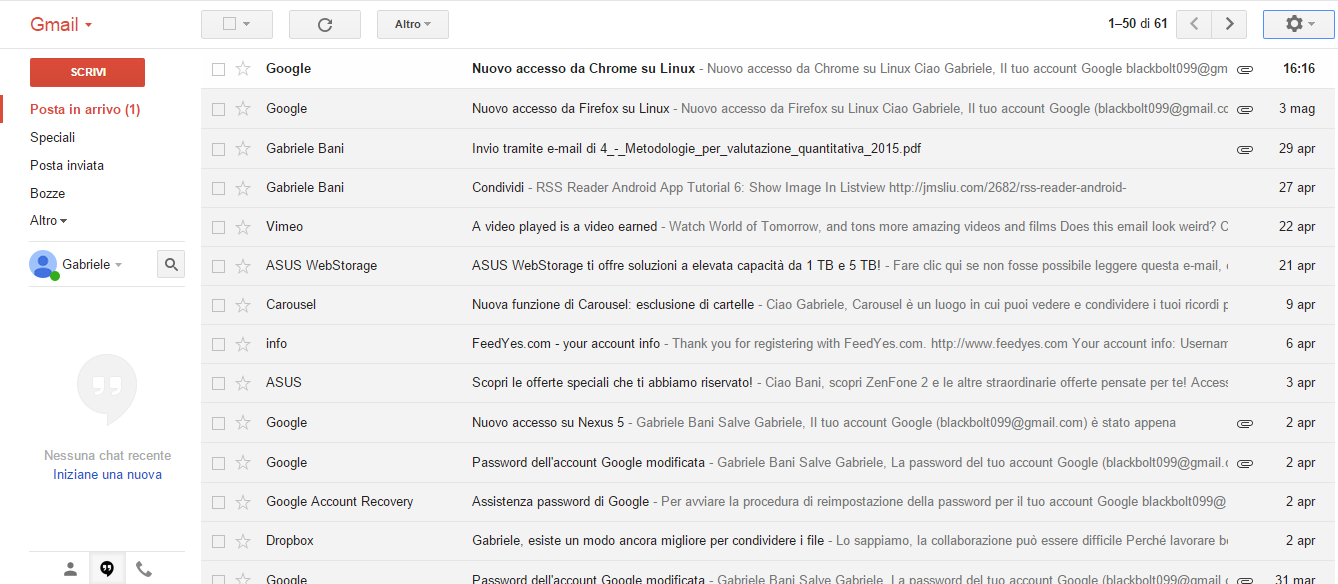
\includegraphics[scale=0.38]{lista_mail_gmail.png}
			\end{center}
			\caption[Elenco mail in Gmail]{L'elenco delle mail visualizzato in Gmail.}
			\label{fig:lista_mail_gmail}
		\end{figure}
		
		Se l'utente lo desidera può modificare, cliccando sull'icona delle impostazioni in alto a destra, la visualizzazione delle mail (es: da ``normale'' ad ``alta'') aumentando, conseguentemente, il numero di mail in ogni pagina e riducendo l'ampiezza di ogni mail.\\
		\\
		In Yahoo Mail la situazione è similare. È sempre possibile, infatti, modificare la quantità di mail visualizzate incrementando o diminuendo l'ampiezza di ogni mail. Tuttavia, se l'utente non provvede a modificare tale schermata, Yahoo Mail inizialmente minimizza l'ampiezza di ogni mail facendo visualizzare all'utente il maggior numero di mail possibili (Figura \ref{fig:lista_mail_yahoo}).
		\begin{figure}[h!]
			\begin{center}
				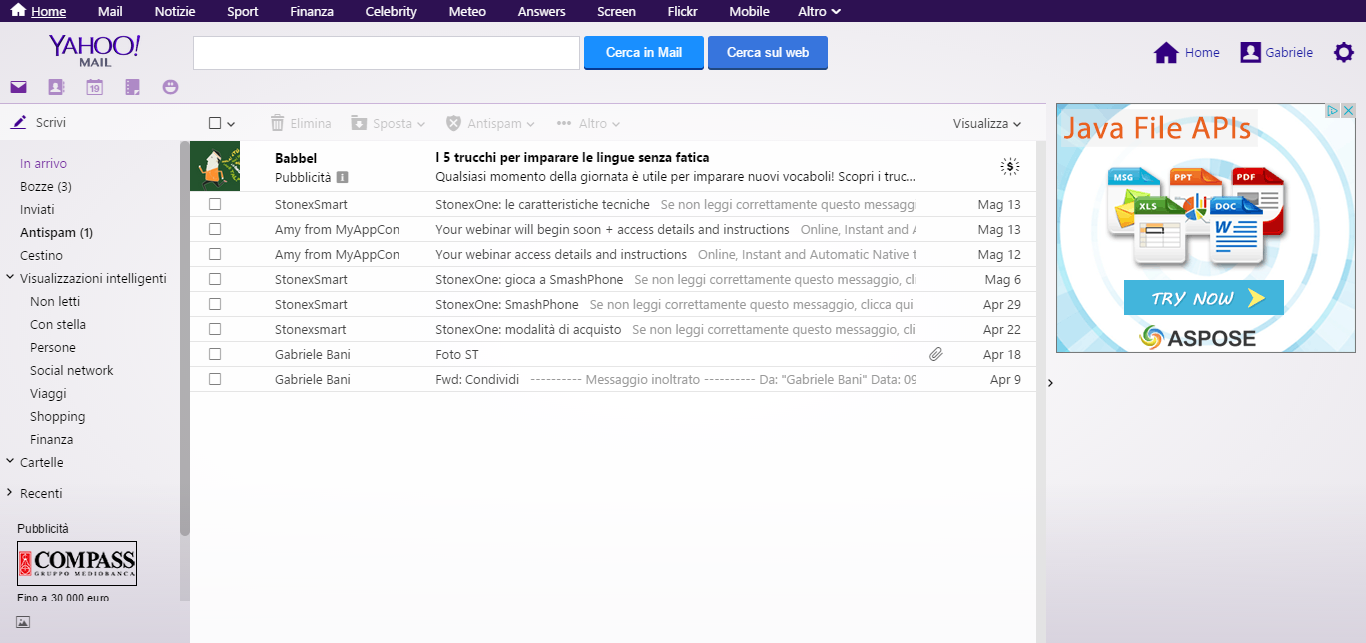
\includegraphics[scale=0.37]{lista_mail_yahoo.png}
			\end{center}
			\caption[Elenco mail in Yahoo Mail]{L'elenco delle mail visualizzato in Yahoo Mail.}
			\label{fig:lista_mail_yahoo}
		\end{figure}
		
		Questa è una scelta in controtendenza rispetto a Gmail.\\
		\\
		I\marginpar{Tooltip} tooltip, ossia i ``consigli'' che appaiono quando il mouse si sposta su uno specifico punto della pagina, sono presenti sia in Gmail che in Yahoo Mail. Tuttavia, in Gmail, non sono presenti i tooltip relativi alle varie mail, ma solo i tooltip relativi al menù (Posta in arrivo, Posta inviata, Spam, …) o alle icone che permettono di eliminare o etichettare una mail, ad esempio. In Yahoo Mail, invece, sono presenti anche i tooltip relativi alle mail, oltre ai tooltip del menù e delle varie icone presenti nella pagina. In particolare, se l'utente si sofferma con il mouse su una specifica mail, allora appare il tooltip contenente l'oggetto della mail, come in Figura \ref{fig:mail_tooltip_yahoo}.
		\begin{figure}[h!]
			\begin{center}
				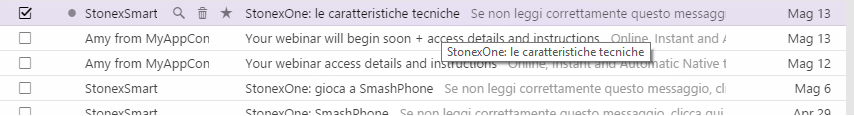
\includegraphics[scale=0.58]{mail_tooltip_yahoo.png}
			\end{center}
			\caption[Tooltip di una mail in Yahoo Mail]{Il tooltip dell'oggetto di una mail in Yahoo Mail.}
			\label{fig:mail_tooltip_yahoo}
		\end{figure}
		
		Tuttavia Gmail implementa dei tooltip dedicati per il mittente di ogni mail, fornendo dettagli aggiuntivi, come la foto. Yahoo Mail, al contrario, visualizza il tooltip del browser dove viene ripetuto il nome del mittente.
		\begin{figure}[h!]
			\begin{center}
				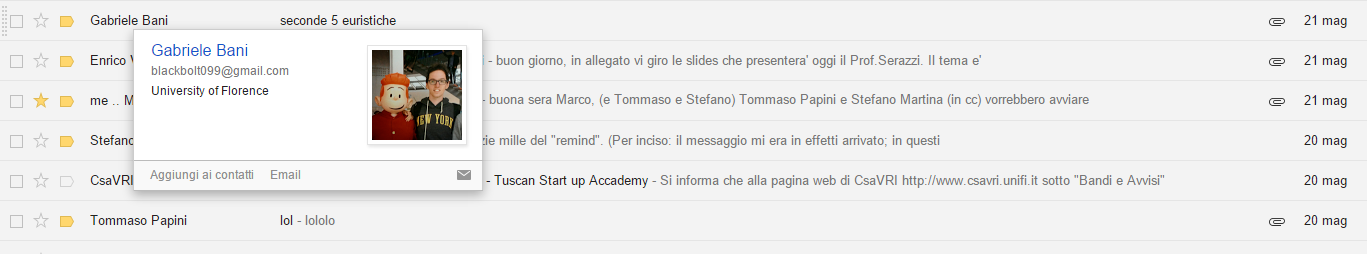
\includegraphics[scale=0.35]{tooltip_mittente_gmail.png}
			\end{center}
			\caption[Tooltip di un mittente in Gmail]{Il tooltip di un mittente di una mail in Gmail.}
			\label{fig:tooltip_mittente_gmail}
		\end{figure}
		
		Gmail\marginpar{Etichette} permette altresì di etichettare le varie mail. È sufficiente, infatti, cliccare sul quadratino a sinistra della mail per selezionare la mail e, successivamente, cliccare sull'icona dell'etichetta che comparirà in alto, scrivendo il nome dell'etichetta che si vuole assegnare alla mail. Nell'esempio in Figura \ref{fig:aggiunta_etichetta_gmail} è stata inserita l'etichetta ``Web'' nelle due mail, mentre in Figura \ref{fig:etichette_gmail} a pagina \pageref{fig:etichette_gmail} vediamo alcuni esempi di etichette a fianco dell'oggetto delle mail.
		\begin{figure}[h!]
			\begin{center}
				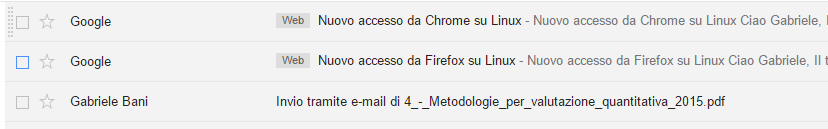
\includegraphics[scale=0.58]{aggiunta_etichetta_gmail.png}
			\end{center}
			\caption[Aggiunta di un'etichetta in Gmail]{L'aggiunta di un'etichetta a due mail in Gmail.}
			\label{fig:aggiunta_etichetta_gmail}
		\end{figure}
		
		Tale funzionalità non viene offerta, invece, da Yahoo Mail.\\
		\\
		Per\marginpar{Da leggere} quanto riguarda, invece, la distinzione tra mail già lette e mail da leggere, possiamo notare come Gmail offra maggiori funzionalità e possibilità di interazione all'utente rispetto a Yahoo Mail. Quest'ultima, infatti, segnala all'utente le mail da leggere solamente utilizzando il ``grassetto''. Gmail, oltre a contraddistinguere le mail da leggere con il grassetto cambia anche lo ``sfondo'' della mail nella schermata principale. Le mail che non sono state ancora lette dall'utente, infatti, sono contraddistinte dal testo in grassetto e dallo sfondo bianco, mentre le mail già lette hanno il testo non in grassetto ed uno sfondo grigio, come vediamo in Figura \ref{fig:nuove_mail_gmail}.
		\begin{figure}[h!]
			\begin{center}
				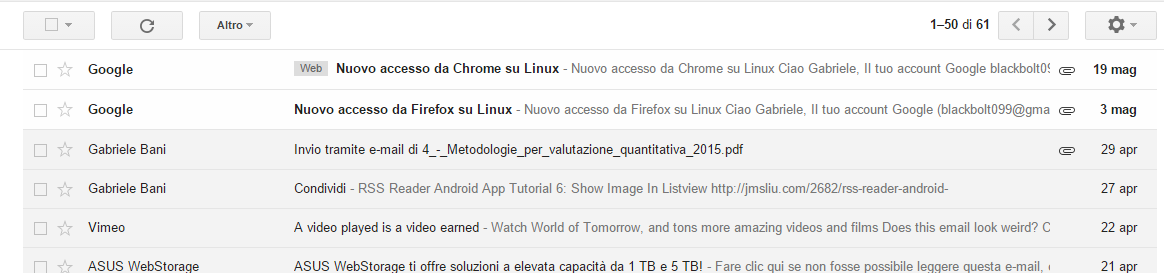
\includegraphics[scale=0.44]{nuove_mail_gmail.png}
			\end{center}
			\caption[Nuove mail in Gmail]{Come vengono visualizzate le nuove mail in Gmail.}
			\label{fig:nuove_mail_gmail}
		\end{figure}
		
		Gmail, inoltre, permette all'utente anche di modificare la schermata di visualizzazione iniziale distinguendo in modo migliore tra mail da leggere e mail già lette, come in Figura \ref{fig:nuove_mail_separate_gmail}.
		\begin{figure}[h!]
			\begin{center}
				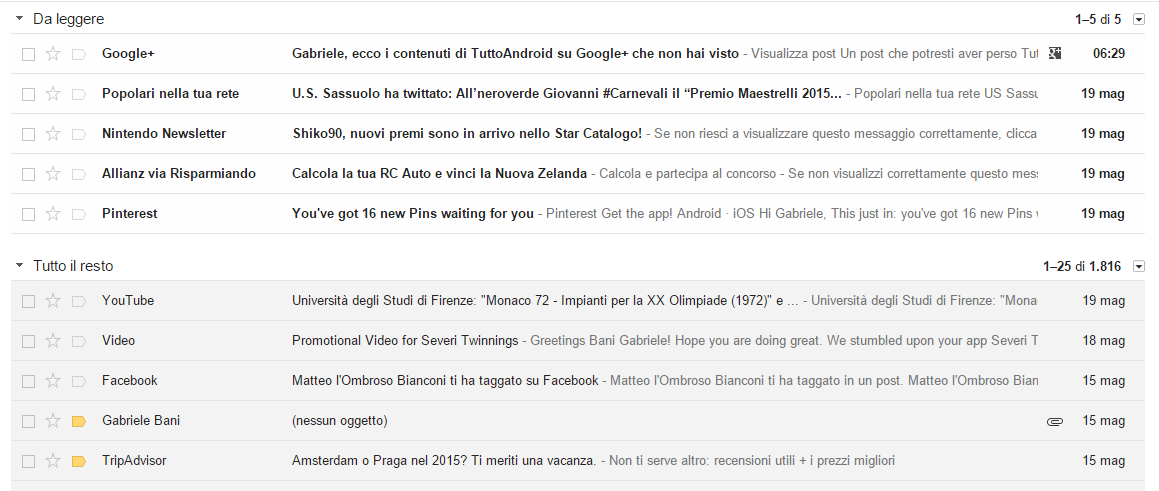
\includegraphics[scale=0.44]{nuove_mail_separate_gmail.png}
			\end{center}
			\caption[Nuove mail in Gmail, liste separate]{Come vengono visualizzate le nuove mail in Gmail utilizzando liste separate.}
			\label{fig:nuove_mail_separate_gmail}
		\end{figure}
		
		\begin{flushleft}
			\begin{tabular}{lr}
				\textsc{Gmail} & $9/10$\\
				\textsc{Yahoo Mail} & $7/10$
			\end{tabular}
		\end{flushleft}
	
	\section{Flessibilit\`{a} d'uso} \label{sec:flessibilità_uso}
	
		Per flessibilità d'uso s'intende che il sito deve:
		\begin{center}
			\begin{minipage}{0.7\textwidth}
				\textit{``Permettere all'utente un uso differenziale, a secondo della sua esperienza, del sito.''}
			\end{minipage}
		\end{center}
	
		Possiamo\marginpar{Preferiti} innanzitutto notare come sia la pagina iniziale che le varie pagine relative alle singole mail possono essere incluse nei ``segnalibri'' (o ``preferiti'') del browser che stiamo utilizzando, indipendentemente dal provider di posta che stiamo utilizzando (Gmail o Yahoo Mail). Tuttavia, Yahoo Mail assegna sempre, come nome del segnalibro, l'username dell'utente Yahoo Mail, non permettendo di distinguere, quindi, differenti segnalibri relativi a pagine differenti della stessa Yahoo Mail. Vediamo due esempi in Figura \ref{fig:preferiti_yahoo}.
		\begin{figure}[h!]
			\begin{center}
				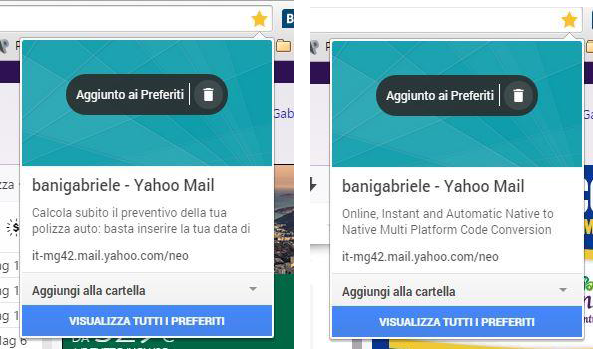
\includegraphics[scale=0.8]{preferiti_yahoo.png}
			\end{center}
			\caption[Preferiti in Yahoo Mail]{Due esempi di pagine di Yahoo Mail aggiunte ai preferiti.}
			\label{fig:preferiti_yahoo}
		\end{figure}
		
		Gmail, invece, assegna come nome del segnalibro il nome della pagina a cui è riferito il segnalibro (Figura \ref{fig:preferiti_gmail}). Se l'utente si trova nella cartella ``Posta in arrivo'', allora il nome del segnalibro sarà ``Posta in Arrivo''. Altrimenti, se l'utente vuole aggiungere una singola mail come segnalibro, allora il nome dell'etichetta sarà l'oggetto della mail a cui si riferisce.
		\begin{figure}[h!]
			\begin{center}
				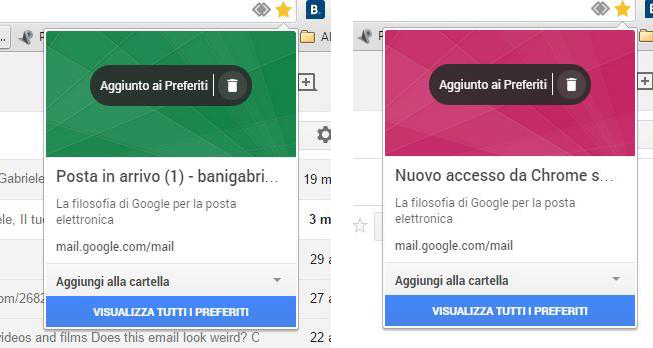
\includegraphics[scale=0.7]{preferiti_gmail.png}
			\end{center}
			\caption[Preferiti in Gmail]{Due esempi di pagine di Gmail aggiunte ai preferiti.}
			\label{fig:preferiti_gmail}
		\end{figure}
		
		Naturalmente, l'utente esperto può modificare opportunamente il nome del segnalibro, ma l'utente neofita del Web si potrebbe trovare in notevole difficoltà a distinguere due segnalibri relativi a pagine differenti della stessa Yahoo Mail. A titolo d'esempio, si veda come in Figura \ref{fig:preferiti_elenco} si possono distinguere tra loro le pagine di Gmail mentre quelle di Yahoo Mail risultano indistinguibili.
		\begin{figure}[h!]
			\begin{center}
				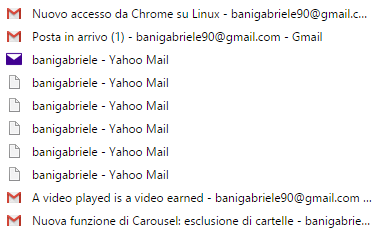
\includegraphics[scale=1]{preferiti_elenco.png}
			\end{center}
			\caption[Lista dei preferiti]{Esempio di lista dei preferiti con pagine di Gmail e Yahoo Mail.}
			\label{fig:preferiti_elenco}
		\end{figure}
		\\
		
		In\marginpar{Ricerca} entrambi i provider di posta è presente anche un campo di ricerca dove poter ricercare le opportune informazioni sia all'interno che all'esterno di Gmail (o Yahoo Mail).\\
		In Gmail è presente il campo di ricerca assieme ad un tasto caratterizzato dalla lente di ingrandimento, che è l'immagine standard per rappresentare il pulsante ``Cerca''. Se l'utente si limita a scrivere la parola chiave nel campo di ricerca e a cliccare sul bottone Cerca, allora verrà effettuata una ricerca all'interno di Gmail, ovvero tra tutte le mail presenti. In alternativa, dopo aver scritto la parola chiave, si può cliccare su ``Cerca <<parola>> nel Web'' ed effettuare, dunque, una ricerca all'esterno di Gmail.
		\begin{figure}[h!]
			\begin{center}
				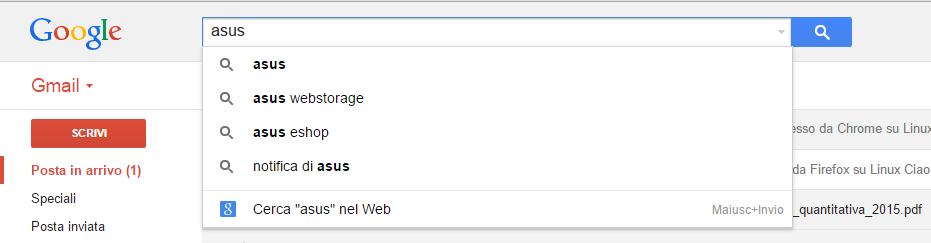
\includegraphics[scale=0.5]{ricerca_gmail.png}
			\end{center}
			\caption[Ricerca in Gmail]{Il motore di ricerca di Gmail.}
			\label{fig:ricerca_gmail}
		\end{figure}
		
		In Yahoo Mail, invece, viene distinta la ricerca all'interno o all'esterno della mail semplicemente tramite l'utilizzo di due bottoni: ``Cerca in Mail'' e ``Cerca sul web''. Dopo aver specificato nel campo di input la parola chiave da ricercare è sufficiente cliccare sul bottone corrispondente per effettuare la ricerca.
		\begin{figure}[h!]
			\begin{center}
				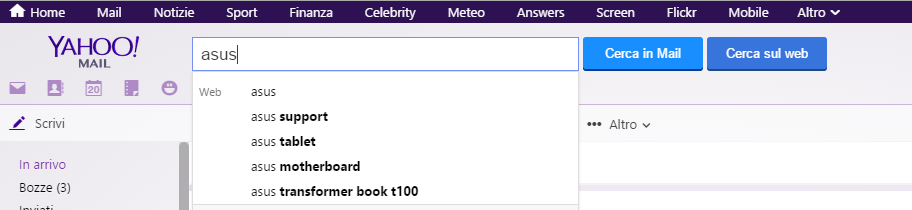
\includegraphics[scale=0.5]{ricerca_yahoo.png}
			\end{center}
			\caption[Ricerca in Yahoo Mail]{Il motore di ricerca di Yahoo Mail.}
			\label{fig:ricerca_yahoo}
		\end{figure}
		\\
		
		In\marginpar{Stile} Gmail, cliccando sull'icona delle impostazioni in alto a destra, è possibile anche modificare lo stile del testo dei messaggi indicando il tipo di carattere, la dimensione ed il colore desiderato.
		\begin{figure}[h!]
			\begin{center}
				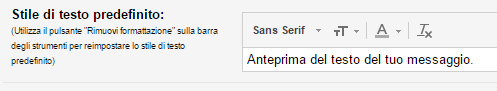
\includegraphics[scale=0.6]{impostazioni_stile_gmail.png}
			\end{center}
			\caption[Impostazioni dello stile in Gmail]{Le impostazioni stilistiche che si possono cambiare in Gmail.}
			\label{fig:impostazioni_stile_gmail}
		\end{figure}
		
		Similmente a Gmail, anche in Yahoo Mail, è possibile modificare le dimensioni del testo cliccando sull'icona delle impostazioni in alto a destra e, successivamente, su ``Impostazioni''. Si aprirà, infatti, la schermata in Figura \ref{fig:impostazioni_stile_yahoo} e sarà sufficiente cliccare su ``Scrivere e-mail'' per modificare il carattere e la dimensione del testo. Rispetto a Gmail, non offre la possibilità di specificare anche il colore del testo desiderato.
		\begin{figure}[h!]
			\begin{center}
				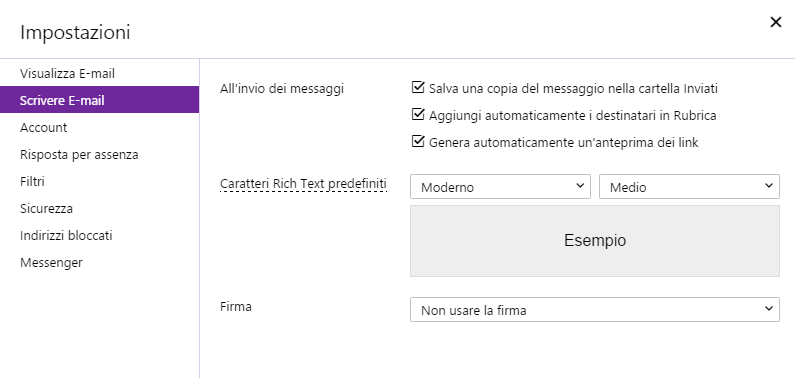
\includegraphics[scale=0.6]{impostazioni_stile_yahoo.png}
			\end{center}
			\caption[Impostazioni dello stile in Yahoo Mail]{Le impostazioni stilistiche che si possono cambiare in Yahoo Mail.}
			\label{fig:impostazioni_stile_yahoo}
		\end{figure}
		\\
		
		In\marginpar{Tasti rapidi} Gmail, dallo stesso menù, è possibile anche attivare le ``scorciatoie da tastiera'' tramite un semplice click. Tuttavia, in Gmail, alcune ``scorciatoie'' sono sempre attive come, ad esempio, l'utilizzo dei tasti freccia per visualizzare un determinato messaggio della cartella Posta in Arrivo, la combinazione di tasti per inviare un messaggio (Ctrl + Invio), per aggiungere destinatari (Ctrl + Maiusc + C), ecc\dots\\
		Se si desiderano, invece, maggiori combinazioni di tasti da utilizzare tramite tastiera come, ad esempio, l'utilizzo di una combinazione di tasti per passare alla conversione meno recente, per tornare all'elenco delle conversazioni, ecc\dots, allora l'utente ha la necessità di attivare le ``scorciatoie da tastiera'' tramite il menù delle impostazioni, in Figura \ref{fig:impostazioni_tasti_rapidi_gmail}. Cliccando su ``Ulteriori informazioni'' si ottengono anche le informazioni su tutte le possibili combinazioni di tasti che è possibile utilizzare.
		\begin{figure}[h!]
			\begin{center}
				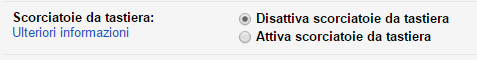
\includegraphics[scale=1]{impostazioni_tasti_rapidi_gmail.png}
			\end{center}
			\caption[Impostazioni dei tasti rapidi in Gmail]{Le impostazioni per i tasti rapidi in Gmail.}
			\label{fig:impostazioni_tasti_rapidi_gmail}
		\end{figure}
		
		In Yahoo Mail, invece, le scorciatoie da tastiera sono già completamente attivate senza bisogno di alcuna interazione da parte dell'utente. Tuttavia, è possibile andare a visualizzare le possibili combinazioni cliccando sull'icona delle impostazioni in alto a destra e poi su ``Tasti di scelta rapida''. Otteremo, infatti, la schermata di riepilogo in Figura \ref{fig:impostazioni_tasti_rapidi_yahoo}.
		\begin{figure}[h!]
			\begin{center}
				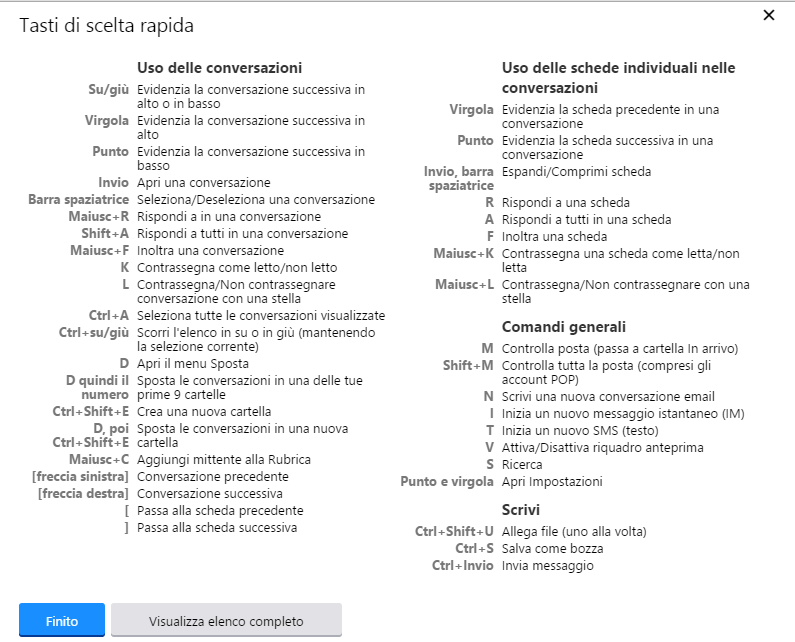
\includegraphics[scale=0.6]{impostazioni_tasti_rapidi_yahoo.png}
			\end{center}
			\caption[Impostazioni dei tasti rapidi in Yahoo Mail]{Le possibili combinazioni di tasti rapidi in Yahoo Mail.}
			\label{fig:impostazioni_tasti_rapidi_yahoo}
		\end{figure}
		\\
		
		Come\marginpar{Etichette} già accennato nelle Sezioni precedenti, Gmail supporta l'utilizzo di etichette mentre Yahoo Mail no. Questa rappresenta una grave mancanza, in termini di flessibilità d'uso, in quando limita l'utente ad assegnare ogni mail ad una e una sola categoria, mentre con Gmail un utente può etichettare una mail con più label e ricercare velocemente una o l'altra categoria.\\
		\\
		Voto finale:
		
		\begin{flushleft}
			\begin{tabular}{lr}
				\textsc{Gmail} & $10/10$\\
				\textsc{Yahoo Mail} & $7/10$
			\end{tabular}
		\end{flushleft}
	
	\section{Design ed estetica minimalista} \label{sec:design_estetica_minimalista}
	
		L'euristica sul design afferma che bisogna:
		\begin{center}
			\begin{minipage}{0.7\textwidth}
				\textit{``Dare più importanza al contenuto che all'estetica.''}
			\end{minipage}
		\end{center}
	
		È\marginpar{Pulsanti} possibile notare subito come i pulsanti siano raggruppati in base alla loro funzione sia in Gmail che in Yahoo Mail. In particolare, i bottoni che contraddistinguono le varie categorie della posta elettronica si trovano sulla sinistra della pagina, mentre i bottoni che permettono, ad esempio, di cancellare, etichettare o segnalare come spam una mail sono tutti presenti in alto al centro della pagina.\\
		I pulsanti meno importanti che operano sulle varie mail sono inizialmente nascosti tramite un'etichetta ``Altro'' in entrambi i provider di posta elettronica.\\
		Differente, invece, è il caso relativo ai pulsanti che contraddistinguono le categorie meno importanti della posta elettronica. Mentre Yahoo Mail, infatti, carica e visualizza immediatamente tutte le varie categorie della propria posta elettronica, Gmail nasconde, almeno inizialmente, le categorie meno importanti della posta. È l'utente, se lo desidera, che provvederà a cliccare su ``Altro'' e ad espandere, dunque, la quantità di pulsanti relativi alle categorie della posta, come vediamo in Figura \ref{fig:menu_yahoo_gmail}.
		\begin{figure}[h!]
			\begin{center}
				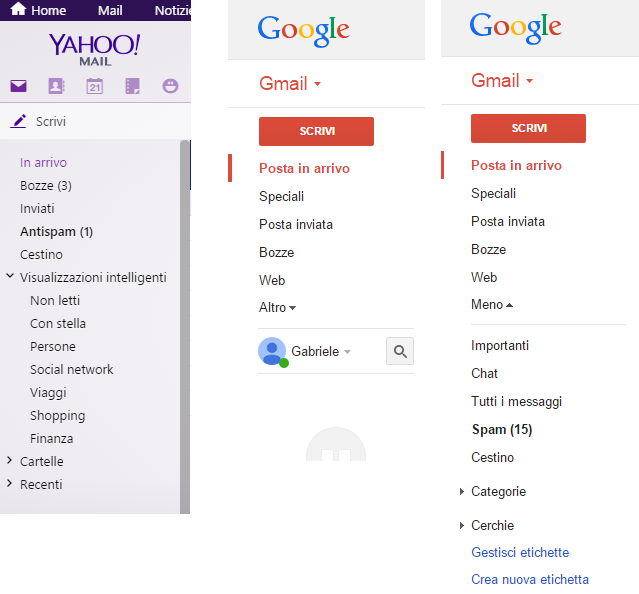
\includegraphics[scale=0.75]{menu_yahoo_gmail.png}
			\end{center}
			\caption[Menù laterale in Yahoo Mail e Gmail]{Comparazione del menù laterale in Yahoo Mail e in Gmail (prima e dopo l'espansione).}
			\label{fig:menu_yahoo_gmail}
		\end{figure}
		\\
		
		I\marginpar{Dettagli} dettagli relativi alle varie mail presenti nella pagina iniziale sono, naturalmente, ridotti al minimo. Nella pagina iniziale di entrambi i provider di posta, infatti, per ogni mail viene fornito solo il mittente, l'oggetto, la data in cui è stata spedita e le prime parole presenti nel testo della mail. Per ulteriori dettagli, l'utente può cliccare sulla mail ed il sistema provvederà ad aprire per intero la suddetta mail.\\
		\\
		Come\marginpar{Da leggere} già accennato precedentemente, Gmail, a differenza di Yahoo Mail, permette anche di suddividere in maniera migliore la lista delle mail presenti, ad esempio, nella cartella Posta in Arrivo. È possibile, infatti, distinguere tra mail ``Da leggere'' e ``Tutto il resto'' (Figura \ref{fig:nuove_mail_separate_gmail} a pagina \pageref{fig:nuove_mail_separate_gmail}).\\
		\\
		Quindi, in conclusione, assegnamo i seguenti voti ai due provider:
		
		\begin{flushleft}
			\begin{tabular}{lr}
				\textsc{Gmail} & $10/10$\\
				\textsc{Yahoo Mail} & $9/10$
			\end{tabular}
		\end{flushleft}
	
	\section{Aiuto all'utente} \label{sec:aiuto_utente}
	
		Il sistema deve:
		\begin{center}
			\begin{minipage}{0.7\textwidth}
				\textit{``Aiutare l'utente a riconoscere, diagnosticare e recuperare l'errore.''}
			\end{minipage}
		\end{center}
	
		Eventuali\marginpar{Destinatario} errori commessi dall'utente possono essere rilevati soprattutto durante la scrittura ed il successivo invio di una mail. L'utente, infatti, potrebbe non aver specificato correttamente o non aver trascritto alcun indirizzo mail del destinatario del messaggio.\\
		In Gmail, se l'utente non ha inserito alcun indirizzo mail del destinatario allora, dopo aver cliccato sul pulsante ``Invia'', compare il messaggio d'errore in Figura \ref{fig:nessun_destinatario_gmail}.
		\begin{figure}[h!]
			\begin{center}
				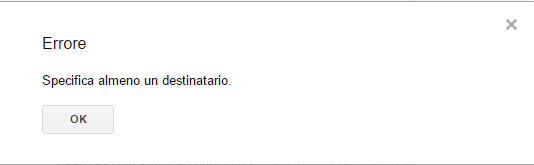
\includegraphics[scale=0.8]{nessun_destinatario_gmail.png}
			\end{center}
			\caption[Errore di nessun destinatario in Gmail]{Errore visualizzato all'invio di una mail senza destinatario in Gmail.}
			\label{fig:nessun_destinatario_gmail}
		\end{figure}
		
		Se l'utente ha, invece, trascritto l'indirizzo mail del destinatario in un formato non corretto (come visto in Figura \ref{fig:errore_indirizzo_gmail} a pagina \pageref{fig:errore_indirizzo_gmail}), allora compare una sottolineatura in rosso all'indirizzo mail durante la scrittura del messaggio. Se quindi clicchiamo sul pulsante ``Invia'' con l'indirizzo sbagliato, compare il messaggio di errore in Figura \ref{fig:formato_indirizzo_gmail}.
		\begin{figure}[h!]
			\begin{center}
				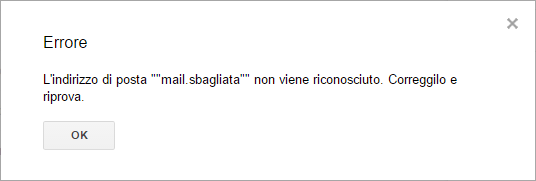
\includegraphics[scale=0.8]{formato_indirizzo_gmail.png}
			\end{center}
			\caption[Errore di indirizzo con formato sbagliato in Gmail]{Errore visualizzato all'invio di una mail con indirizzo di formato scorretto in Gmail.}
			\label{fig:formato_indirizzo_gmail}
		\end{figure}
		
		In Yahoo Mail, invece, il messaggio di errore, sia in caso di mancata trascrittura dell'indirizzo mail del destinatario che in caso di scrittura non corretta dell'indirizzo, è sempre quello in Figura \ref{fig:nessun_destinatario_yahoo}.
		\begin{figure}[h!]
			\begin{center}
				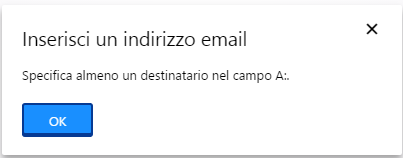
\includegraphics[scale=1]{nessun_destinatario_yahoo.png}
			\end{center}
			\caption[Errore di destinatario in Yahoo Mail]{Errore visualizzato all'invio di una mail senza destinatario o con destinatario con formato scorretto in Yahoo Mail.}
			\label{fig:nessun_destinatario_yahoo}
		\end{figure}
		
		Tuttavia, se l'utente ha inserito come indirizzo mail del destinatario un indirizzo di formato scorretto, come ``mail.sbagliata'', allora il messaggio di errore non è appropriato. L'utente, infatti, ha provveduto ad inserire un destinatario nel campo A, anche se non è stato trascritto in modo corretto. Il messaggio di errore, dunque, dovrebbe essere differente dal caso in cui non sia stato specificato alcun indirizzo mail nel destinatario del messaggio.
		
		\begin{flushleft}
			\begin{tabular}{lr}
				\textsc{Gmail} & $10/10$\\
				\textsc{Yahoo Mail} & $7/10$
			\end{tabular}
		\end{flushleft}
	
	\section{Documentazione} \label{sec:documentazione}
	
		Infine, l'ultima euristica di Nielsen afferma che:
		\begin{center}
			\begin{minipage}{0.7\textwidth}
				\textit{``Anche se un sito dovrebbe essere navigabile senza documentazione, è preferibile che essa sia disponibile.''}
			\end{minipage}
		\end{center}
	
		Il materiale di aiuto (denominato anche ``Documentazione'') viene fornito in modo differente nei due provider di posta elettronica (Gmail e Yahoo Mail).\\
		\\
		In Gmail, dopo aver cliccato sull'icona delle impostazioni e, successivamente, su ``Guida'', appare una nuova finestra denominata ``Guida di Gmail'' (Figura \ref{fig:guida_gmail}) che si sovrappone alla schermata precedente della posta elettronica.
		\begin{figure}[h!]
			\begin{center}
				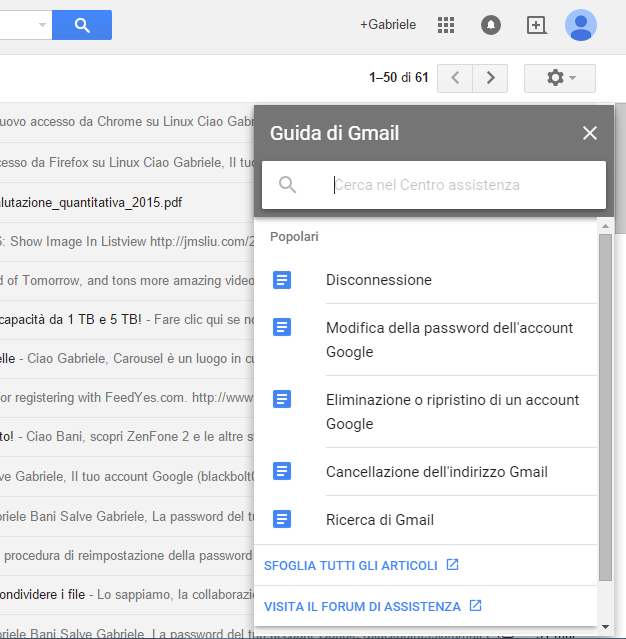
\includegraphics[scale=0.6]{guida_gmail.png}
			\end{center}
			\caption[Guida di Gmail]{La guida agli utenti di Gmail.}
			\label{fig:guida_gmail}
		\end{figure}
		
		Tale finestra è caratterizzata da un campo di input, dove è possibile scrivere che cosa l'utente sta effettivamente cercando, e da alcuni suggerimenti che propone il sistema. L'utente, inoltre, può anche provvedere a spostare in un'altra parte dello schermo tale finestra, semplicemente effettuando un'operazione di trascinamento.\\
		La ``Guida di Gmail'', quindi, permette all'utente sia di rimanere nella pagina di posta elettronica dove si trovava precedentemente ma, al contempo, anche di ricercare eventuali informazioni o chiarimenti su alcune operazioni inerenti alla gestione dell'account di posta.\\
		\\
		Anche Yahoo Mail ha un opportuno meccanismo di documentazione. Per poter accedere a tale materiale, è sufficiente cliccare sull'icona delle impostazioni in alto a destra e, successivamente, sull'etichetta ``Aiuto''. Il sistema provvederà ad aprire una nuova pagina dove l'utente potrà cercare l'informazione desiderata.
		\begin{figure}[h!]
			\begin{center}
				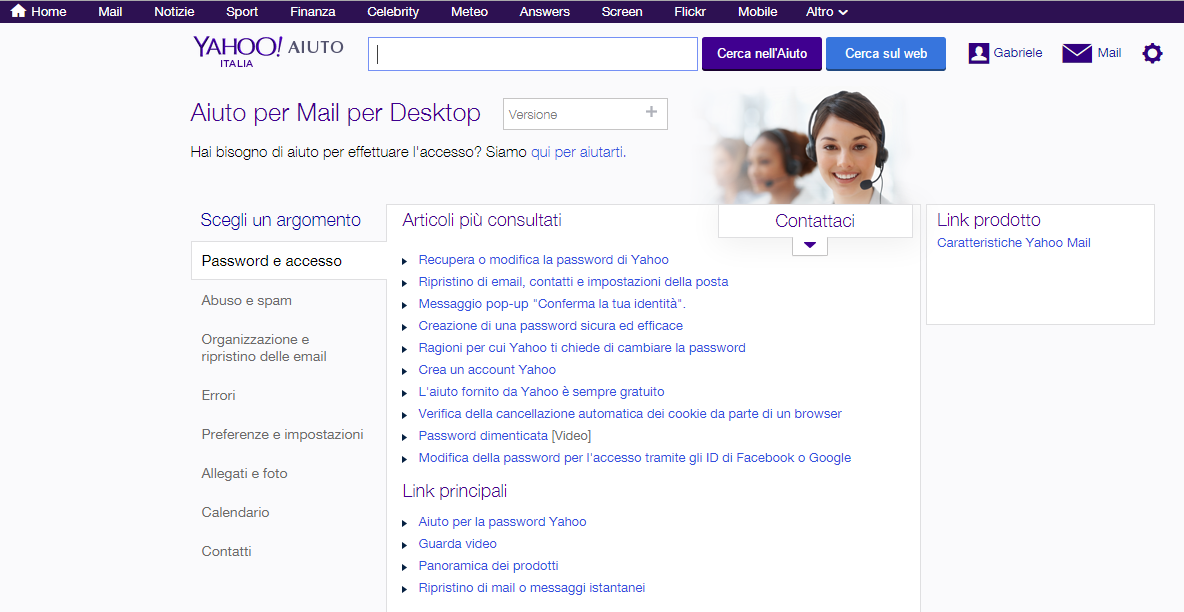
\includegraphics[scale=0.4]{guida_yahoo.png}
			\end{center}
			\caption[Guida di Yahoo Mail]{La guida agli utenti di Yahoo Mail.}
			\label{fig:guida_yahoo}
		\end{figure}
		
		Tuttavia, mentre in Gmail l'accesso alla documentazione non escludeva la permanenza nell'account di posta elettronica, in Yahoo Mail l'accesso al materiale di aiuto presuppone di lasciare la pagina precedente, risultando più intrusiva e a volte anche scomoda.
		
		\begin{flushleft}
			\begin{tabular}{lr}
				\textsc{Gmail} & $10/10$\\
				\textsc{Yahoo Mail} & $8/10$
			\end{tabular}
		\end{flushleft}
		
	\section{Valutazione finale} \label{sec:valutazione_finale}
	
		Tirando le somme su quanto visto in questo capitolo, possiamo dire che sia Gmail che Yahoo Mail sono caselle di posta elettronica molto usabili e ben strutturate.\\
		\\
		Gmail è risultato, in generale, più usabile in quanto ha curato di più l'aspetto e i dettagli dell'interfaccia con cui l'utente dovrà poi interagire. Questo non toglie niente a Yahoo Mail, che rimane un sito validissimo, funzionante e ben strutturato. Tuttavia non potevamo assegnare lo stesso voto sia a Gmail che a Yahoo Mail in quanto quest'ultimo ha tralasciato alcuni dettagli che Gmail ha invece preso in considerazione.\\
		\\
		In Figura \ref{fig:valutazione_euristica} proponiamo due grafici riassuntivi della valutazione di usabilità per Gmail e Yahoo Mail secondo le 10 euristiche.
		\begin{figure}[h!]
			\begin{center}
				\subfloat[][Line chart]{
					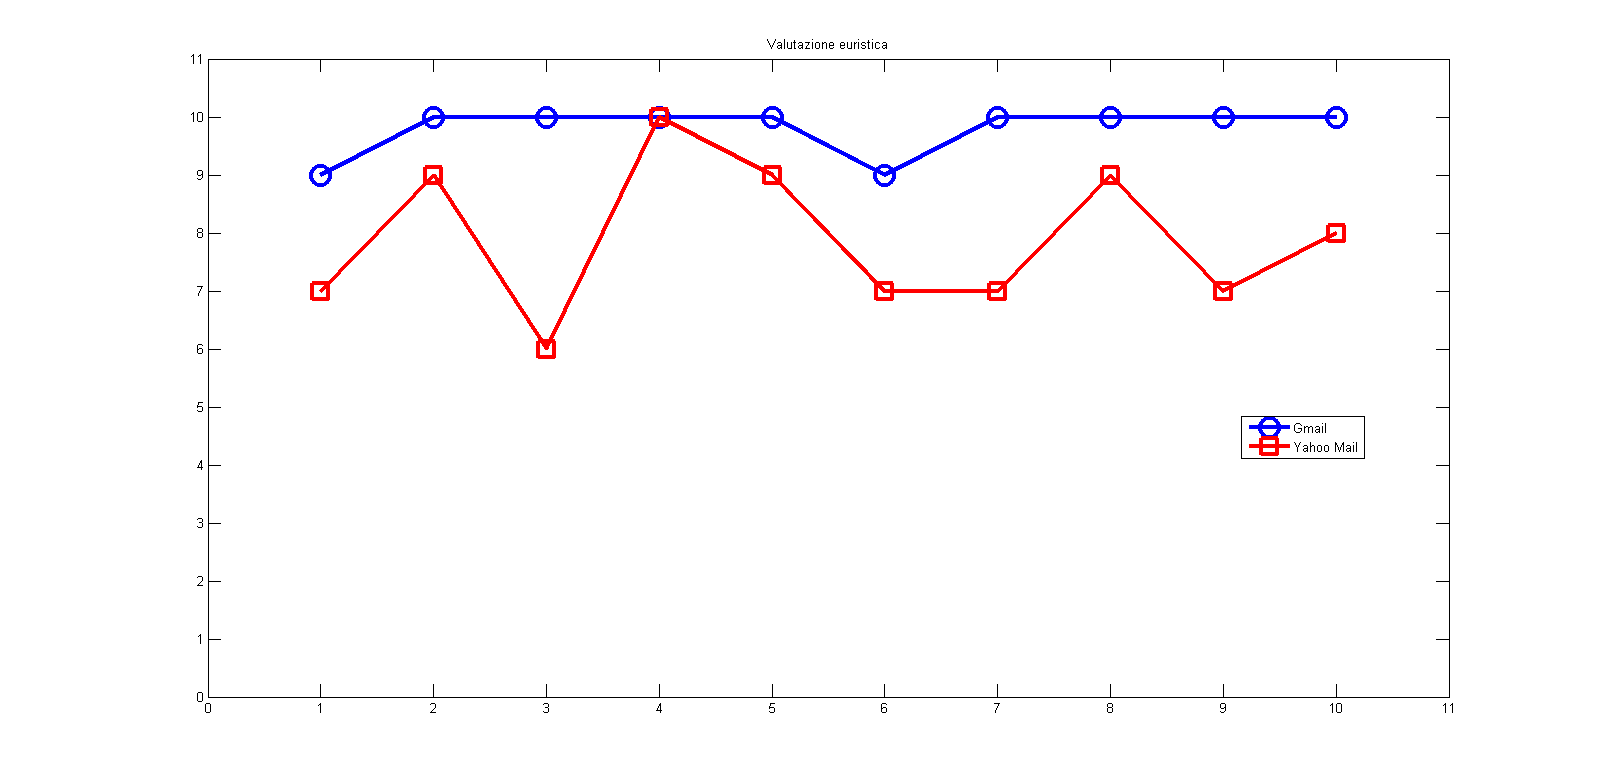
\includegraphics[scale=0.3]{valutazione_euristica_line.png}
				}\\
				\subfloat[][Radar chart]{
					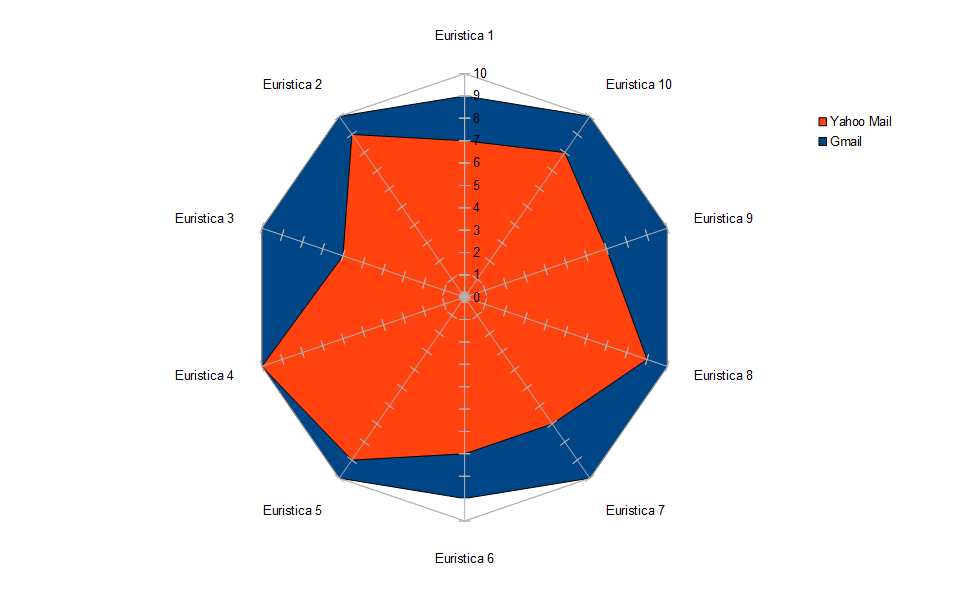
\includegraphics[scale=0.4]{valutazione_euristica_radar_filled.png}
				}
			\end{center}
			\caption[Grafici della valutazione euristica]{Grafici riassuntivi dove viene comparata la valutazione euristica per Gmail e Yahoo Mail.}
			\label{fig:valutazione_euristica}
		\end{figure}
		\\
		
		Detto questo, facciamo una media dei voti assegnati per le varie euristiche ed assegnamo un voto finale di usabilità ai due provider.
		
		\begin{flushleft}
			\begin{tabular}{lr}
				\textsc{Gmail} & $9.8/10$\\
				\textsc{Yahoo Mail} & $7.9/10$
			\end{tabular}
		\end{flushleft}
		